%%%%%%%%%%%%%%%%%%%%%%%%%%%%%%%%%%%%%%%%%
% Cheatsheet
% LaTeX Template
% Version 1.0 (12/12/15)
%
% This template has been downloaded from:
% http://www.LaTeXTemplates.com
%
% Original author:
% Michael Müller (https://github.com/cmichi/latex-template-collection) with
% extensive modifications by Vel (vel@LaTeXTemplates.com)
%
% License:
% The MIT License (see included LICENSE file)
%
%%%%%%%%%%%%%%%%%%%%%%%%%%%%%%%%%%%%%%%%%

%----------------------------------------------------------------------------------------
%	PACKAGES AND OTHER DOCUMENT CONFIGURATIONS
%----------------------------------------------------------------------------------------

\documentclass[11pt]{scrartcl} % 11pt font size

\usepackage[utf8]{inputenc} % Required for inputting international characters

\usepackage[margin=1cm, landscape]{geometry} % Page margins and orientation

\usepackage{graphicx} % Required for including images

\usepackage{color} % Required for color customization
\definecolor{mygray}{gray}{.75} % Custom color

\usepackage{url} % Required for the \url command to easily display URLs

\usepackage{amsmath}

\usepackage[ % This block contains information used to annotate the PDF
colorlinks=false,
pdftitle={Orbiter 2016 - Keyboard Cheat Sheet},
pdfauthor={Jan Wedekind},
pdfsubject={Cheat sheet for Orbiter 2016},
pdfkeywords={Orbiter, Cheatsheet}
]{hyperref}

\setlength{\unitlength}{1mm} % Set the length that numerical units are measured in
\setlength{\parindent}{0pt} % Stop paragraph indentation

\renewcommand{\dots}{\ \dotfill{}\ } % Fills in the right amount of dots

\newcommand{\command}[2]{\texttt{#1}~\dotfill{}~#2\\} % Custom command for adding a shorcut

\newcommand{\sectiontitle}[1]{\paragraph{#1} \ \\} % Custom command for subsection titles

\newcommand{\sep}{\hspace{5mm}}

%----------------------------------------------------------------------------------------

\begin{document}
\section*{Orbiter 2016 -- Keyboard Cheat Sheet} % Title

\begin{minipage}[t]{64mm}
\sectiontitle{Game Play}
\command{F1}{toggle external view}
\command{Ctrl + F1}{camera dialog}
\command{Alt + F1}{help window}
\command{Ctrl + F2}{time lapse dialog}
\command{F3}{vessel dialog}
\command{Ctrl + F3}{previous vessel}
\command{F4}{main menu}
\command{Ctrl + F4}{custom functions dialog}
\command{Alt + F4}{exit}
\command{Ctrl + F5}{record/playback dialog}
\command{F9}{toggle planetarium}
\command{Ctrl + F9}{planetarium dialog}
\command{T}{time lapse}
\command{R}{real time}
\command{I}{toggle info display}
\command{Ctrl + I}{object info dialog}
\command{Ctrl + M}{map dialog}
\command{Ctrl + P}{pause}
\command{Ctrl + S}{quick save}

\sectiontitle{External Camera}
\command{Ctrl + $\downarrow\uparrow\rightarrow\leftarrow$}{camera rotation}
\command{pg up/pg dn}{increase/decrease distance}
\command{F2}{toggle tracking mode}

\sectiontitle{Cockpit Camera}
\command{$\downarrow\uparrow\rightarrow\leftarrow$}{scroll panel}
\command{Ctrl + $\downarrow\uparrow\rightarrow\leftarrow$}{switch to other panel}
\command{Alt + $\downarrow\uparrow\rightarrow\leftarrow$}{view direction}
\command{Home}{default viewing direction}
\command{F8}{toggle cockpit views}
\command{X}{zoom out}
\command{Z}{zoom in}
\end{minipage}
\sep
\begin{minipage}[t]{64mm}
\sectiontitle{Actuators}
\command{Ctrl + A}{auxiliary power unit}
\command{Ctrl + D}{undock}
\command{Ctrl + K}{nose cone}
\command{Ctrl + V}{hover doors}
\command{Ctrl + O}{outer airlock}
\command{Ctrl + Y}{cabin hatch}
\command{Alt + R}{radiator}
\command{Ctrl + $\backslash$}{retro doors}
\command{G}{gear}
\command{,/.}{left/right wheel brake}

\sectiontitle{Thrusters Numpad}
\command{Num +}{full main}
\command{Num -}{full retro}
\command{Num *}{kill retro and main}
\command{Ctrl + Num +}{increase main}
\command{Ctrl + Num -}{decrease main}
\command{Num 0}{increase hover}
\command{Num .}{decrease hover}
\command{Ctrl + *}{kill hover}
\command{Ctrl + Num /}{enable/disable RCS}
\command{Num /}{toggle rotation/translation}
\command{Num 2/8}{up/down}
\command{Num 1/3}{left/right}
\command{Num 6/9}{forward/backward}
\command{Ctrl + Num 2/8}{up/dn 10\% thrust}
\command{Ctrl + Num 1/3}{left/right 10\%}
\command{Ctrl + Num 6/9}{forw/bckwd 10\%}
\command{Num 5}{kill rotation}
\command{A}{auto hover}
\command{L}{auto level}
\command{[/]}{turn prograde/retrograde}
\command{;/'}{turn orbit-normal/antinormal}
\end{minipage}
\sep
\begin{minipage}[t]{64mm}
\sectiontitle{Aerodynamic Controls}
\command{Alt + Num /}{enable/disable}
\command{Num 4/6}{bank}
\command{Num 2/8}{pitch}
\command{Num 1/3}{yaw}
\command{Ins/Delete}{trim}

\sectiontitle{HUD}
\command{Ctrl + H}{on/off}
\command{Alt + H}{toggle colour}
\command{Alt + X}{increase brightness}
\command{Alt + Z}{decrease brightness}
\command{H}{toggle surface/orbit/dock}
\command{Ctrl + R}{reference}
\command{Ctrl + Alt + R}{ref. (subset)}

\sectiontitle{XR Series}
\command{0, 1, $\ldots$, 9}{Multi Display Area}
\command{Alt + ,}{shift center of gravity aft}
\command{Alt + .}{shift center of gravity fwd}
\command{Ctrl + ,}{increase elevator trim}
\command{Ctrl + .}{decrease elevator trim}
\command{Alt + M}{re-center center of gravity}
\command{Alt + J}{toggle XR5 RCS config}
\command{Alt + S}{airspeed hold autopilot}
\command{Ctrl + B}{air brake}
\command{Ctrl + G}{scram doors}
\command{Ctrl + W}{reset alarm}
\command{Alt + Num +}{increase scram}
\command{Alt + Num -}{decrease scram}
\command{Ctrl + Backspace}{kill scram}
\command{Space}{disengage autopilot}
\command{Alt + ;}{main/scram gimbal up}
\command{Alt + L}{main/scram gimbal right}
\command{Alt + P}{main/scram gimbal down}
\command{Alt + '}{main/scram gimbal left}
\command{Alt + 0}{gimbal re-center}
\end{minipage}
\sep
\begin{minipage}[t]{64mm}
\sectiontitle{Important Addons}
D3D9Client
OrbiterSound
DeltaGliderIV
UCGO30
HUDDrawerSDK
ModuleMessagingExt
BaseSync
TransX
AeroBrake
LaunchMFD
GlideSlope
BurnTimeCalculator
DeltaGliderXR1
XR2Ravenstar
XR5Vanguard
ISS\\

\vspace{\baselineskip}
\sectiontitle{Links and information}
\url{http://orbit.medphys.ucl.ac.uk/download/orbiter.pdf}\medskip\\
\url{http://orbiter.dansteph.com/forum/index.php?page=download}\medskip\\
\url{http://www.orbithangar.com/}\medskip\\
\url{http://www.alteaaerospace.com/}\medskip\\
\url{https://www.orbiter-forum.com/}\medskip\\

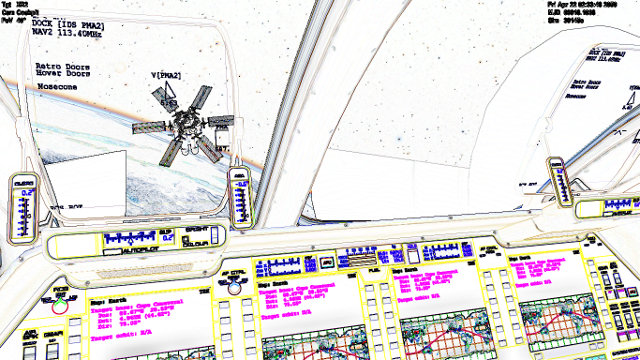
\includegraphics[width=\textwidth]{docking}

\linethickness{0.5mm} % Thickness of the footer line
{\color{mygray}\line(1,0){30}} % Print the line with a custom color

\footnotesize{
Created by Jan Wedekind, 2017\\
\url{http://www.wedesoft.de/}\\
}

\end{minipage} % End the third column of text

\end{document}
